\section{Development}

\subsection{Introduction}
In this section, I will discuss the development process of the domain project.  There will be six sections, each exploring the six main features established in the requirement section, which are declaration of domains, assignment of signatures to function/methods, declaration of variables, combination of domains, implicit conversions of variables, and type checking at compile time. 

\subsection{Declaration of domains}
The first feature  I have implemented was declaration of domains.  There are several methods and classes that are relevant to the code, which will be discussed one by one.  
\begin{lstlisting}[caption={Method for creating domains}]
def create_domain(compound: 0, name: "")
    if !block_given? && compound == 0
        raise ArgumentError.new "No block of rules were given.  There must be at least one rule for the domain"
    end

    cl = Class.new do
       extend DomainClass   
        include DomainClass
    end

    prev = @domain_created

    @domain_created = cl

    @domain_created.compound_domain = unless compound == 0 then compound else @domain_created end
    @domain_created.rules = {}
    @domain_created.translators = {}
    @domain_created.default = nil
    @domain_created.translation_map = {}

    yield if block_given?
        
    @domain_created.translators.each_key do |key|
        d_in, d_out = key

        if !@domain_created.translation_map.has_key? d_in
            @domain_created.translation_map[d_in] = []
        end

        @domain_created.translation_map[d_in] << d_out
    end

    @domain_created = prev

    cl.send :generate_translators

    if not name.empty?
        if self.inspect == 'main'
            Object.const_set(name, cl)
        else
            self.const_set(name, cl)
        end
    else
        return cl
    end
end
\end{lstlisting}

The first of the relevant methods is create\_domain.  This method is simple compared to some of the TracePoint driven methods that will appear in the later codes.  First, the code checks to see if there are any rules with the provided domain.  This is done to prevent users from create a domain that lacks any rules.  Next, the method creates an anonymous class that implements DomainClass, which is a module that contains various basic functions for domains to function, which will be shown in Figure 2. Next, an instance varialbe @domain\_created is stored in prev variable.  This is because the @domain\_created variable is basically a global variable for the create\_domain method, and if another domain was declared within the block, the value can be overridden with the new domain.  To prevent this, prev store the value @domain\_created was previously and return it to the original value after the domain is created.  After prev has been set, the anonymous class is assigned to @domain\_created and all important values such as rules and translation rules are initiated.  The block is then yielded to read all the rules inside, and saved to the hashes. The lines 23 to 35 will be explained in detail in the later sections, as it is more relevant there.  Finally, the anonymous class is given a name and is defined in the appropriate classes as a constant. 

\begin{lstlisting}[caption={Domain module}]
module DomainClass
    include DomainErrors
    attr_accessor :rules
    attr_accessor :translators
    attr_accessor :compound_domain
    attr_accessor :default
    attr_accessor :translation_map

    def print_rules; end

    def print_translators; end

    def value?(value); end

    def check_rules(rules, value); end

    def translate(d_in, d_out, value); end

    def value=(value); end

    def value(domain=nil); end
end
\end{lstlisting}

DomainClass module is the next set of codes that will be discussed.  This module contains various different methods a domain should have to function properly.  The implementations for each of the methods are omitted to prevent codes from taking too much space and because they are mostly self-explanatory.  The most important methods are value?, value=, and value.  value? method checks the value in the argument to make sure the argument follows the rules of the domain.  check\_rules in the module is the private helper method for the value? method.  value= assigns the value to the domain for domain to use in the future, which can be read through the value method.  Domain should also have ways to translate from one domain to another, which is used in implicit conversions.

\begin{lstlisting}[caption={Monkey patching Object class}]
class Object
    class << self
        include Util
        def rules
            [{ self => Proc.new { |x| true } }]
        end

        def compound_domain
            self
        end

        def translators
            {}
        end

        def value?(x)
            return x.is_a? self
        end

        def has_compound_domain
            self != compound_domain
        end

        def method_added(m)
            super
        end

        def singleton_method_added(m)
            super
        end

        make_compound_domain :+
        make_compound_domain :-
        make_compound_domain :&

        alias :union :+
        alias :intersect :&
        alias :difference :-
    end

    def part_of?(x)
        if x.singleton_methods.include? :value?
            x.value? self
        end

        raise TypeError.new("#{x} is not a domain.")
    end

    def value
        return self
    end
end
\end{lstlisting}

Finally, the domain adds new methods to Object class so that all class behave similarly to the domains, as type is a subset of domain in type checking sense.  This allows classes that already exist, such as Integer and String class, act similarly to the domain, which allows the program to treat them like one for various benefits such as the combination of domains.

Through these methods, the users of this library can create domain using syntax like this:

\begin{lstlisting}[caption={Sample code: declaration of domains}]
def is_integer(x)
    return Integer(x) rescue false
end

domain :Int do
    rule(Integer)
    rule(String) { |x| is_integer?(x) }
end
\end{lstlisting}

The domain :Int do \ldots end defines domain Int with two rules.  The first rule states that it can accept any Integer, and the second rule states that if the object is String, domain Int can accept values that returns true for the is\_integer?() method, which checks if the x is an integer.  With this domain, it is possible to use both integer and string only containing integer as if they're integer, which can be a very power tool.

\subsection{Assignment of signatures to function/methods}

Unlike the declaration of domain, the implementation of signatures require heavy exploitation of Ruby's metaprogramming features, which can be difficult to understand.  Additionally, the implementation is very long, so it requires extensive explanation on how they are implemented.

The signature is implemented in three steps.  First, the signature reads the String passed in as a signature and parse and interpret the string to see if the String is a valid signature.  The string is then transformed into two arrays, each indicating the rules for argument and rules for return values respectively.  The arrays are then used to wrap the new method with checks that makes sure the argument and return value conforms to the rules and the original method is overridden with the new wrapped method.  We will discuss each parts in detail over this section

\begin{lstlisting}[caption={Parser method}]
def parse_tokens(sig)
    valid_tokens = ['(', ')', ',', '[', ']', '$', '{', '}', '&']
    sig.gsub!(/\s/, "")

    tokens = []

    other = ""
    token = ""

    state = :default
    redo_state = false

    sig.each_char do |x|
        case state
        when :default
            token += x
            case x
            when '*'
                state = :star
            when '-'
                state = :arrow
            when *valid_tokens
                state = :accepted
            else
                state = :other
            end
        when :star
            case x
            when '*'
                state = :accepted
                token += x
            else
                state = :accepted
                redo_state = true
            end
        when :arrow
            token += x
            case x
            when '>'
                state = :accepted                   
            else
                state = :other
            end
        end

        if state == :other
            other += token
                
            if token == ":" then state = :accepted else state = :default end
            token = ""
        end
            
        if state == :accepted
            if !other.empty? then tokens << other; other = "" end
            tokens << token if !token.empty?
            token = ""
            state = :default
        end

        if redo_state
            state = :default
            redo_state = false
            redo
        end
    end

    tokens << other if !other.empty?
    tokens
end
\end{lstlisting}

First, this method parses the string into list of tokens that can be used to interpret what it means.  The method follows the following finite state machine to parse the string:

\begin{figure}[H]
\caption{Finite State Machine}
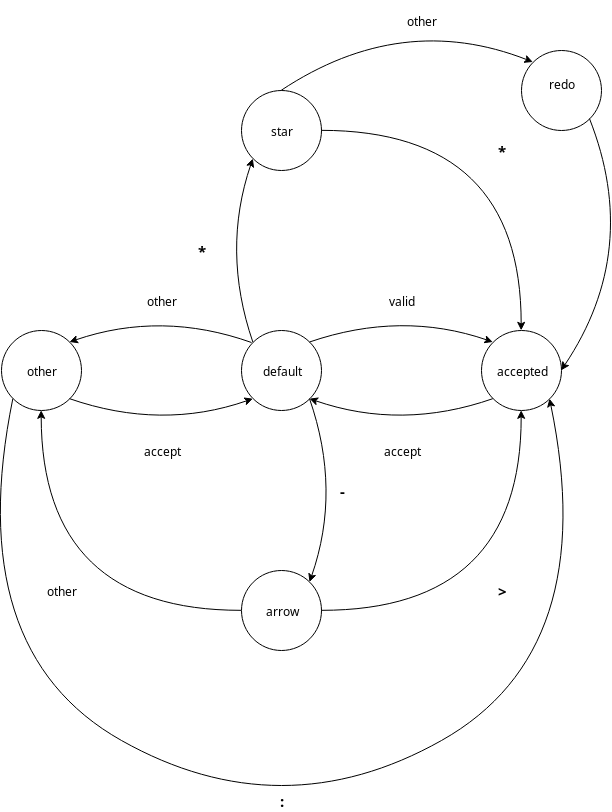
\includegraphics[width=10cm]{diagram_fsm}
\centering
\end{figure}

The machine begins at default, and moves to star state when it finds a {*} symbol, arrow state ({-}\textgreater) when it finds the {-} symbol, accepted state when it finds any of the valid tokens defined in the array, and other state for any other symbols.  On star state, it moves to accepted state when it finds another {*} symbol and redo state otherwise, which is a state that quickly moves to accepted state and re-examine the current symbol.  The arrow state changes to accepted state only when it finds the \textgreater symbol which completes the arrow.  The remaining other symbols move to other state.  Other state simply concatenates the value to a variable, and if {:} was found, Other moves to accepted state to save it as a keyword.  On accepted state, the tokens that has been found is stored in an array.  After the entire string has been parsed, the array is returned.

\begin{lstlisting}[caption={Interpreter method}]
def interpret_tokens(cl, local, tokens)
    # Get tokens for arg and return separated

    k = tokens.slice_after { |x| x == '->' }.to_a
    a, r = k
    a.pop
    length = k.length

    if length != 2
        raise ArgumentError.new "Expected only one arrow (->), got #{length - 1}"
    end

    # Change the list of tokens into something more usable

    # Ignore the () if it's properly at the begnning and end
    a = a[1..-2] if a[0] == '(' && a[-1] == ')'
    r = r[1..-2] if r[0] == '(' && r[-1] == ')'

    a = retrieve_tokens(cl, local, a)
    r = retrieve_tokens(cl, local, r)[0]

    return a, r
end
\end{lstlisting}

Now that all the tokens are in array, the next step is to store them into two arrays, one for argument and another for return values.  Once the tokens are separated, it is sent to retrieve token method, which will turn all the tokens into something the wrapper can use to check the values.

\begin{lstlisting}[caption={Retriever method}]
def retrieve_tokens(cl, local, tokens)
    # initialization

    tokens.each do |x|
        case state
        when :token
            case x
            when '['
                # array logic
            when '{'
                # hash logic
            when ',', ']', '}'
                # error
            when '*', '**'
                # star logic
            when '$'
                # optional logic
            when '&'
                # block logic
            else
                # non-token logic
        when :comma
            # comma logic
        end
    end
    return arg, kwarg
end
\end{lstlisting}

The retrieve\_token method can be generalized through this code.  After initializing important variables, the method iterates through all the tokens that are given, and performs different checks to see what the token means.  There are two states in this method, which are ``token'' and ``comma''.  Because the tokens alternate between valid token and comma in real code, this two states are alternated between each other to make sure all tokens separated by comma means something.

\begin{lstlisting}[caption={Wrapper method: overview}]
def wrap_method(signature)
    # initialize

    return_trace = TracePoint.new(:return) do |tp|
        # parse signature
	# initialization for the new method
	# check if the method has correct argument(s)
	# wrap the method with checks and replace it
	# add it to the correct place and with right scope
    end

    line_trace = TracePoint.trace(:line) do |tp|
    	# get a binding
	# enable return_trace and disable line_trace
    end
end
\end{lstlisting}

Next, the wrapper method uses the established parser in order to wrap the method correctly.  Because this method is large, all logic will be separated into multiple sections to explain them all in detail.

\begin{lstlisting}[caption={Wrapper method: check if the method has correct argument(s)}]
return_trace = TracePoint.new(:return) do |tp|
    # ...
    # Check for validity of the method by getting its arity and aligning it with the length of arguments in signature
    method = tp.self.instance_method(method_name) if tp.method_id == :method_added
    method = tp.self.method(method_name) if tp.method_id == :singleton_method_added

    # Check if the parameters should have star variable (*arg) or double star variable (**arg)
    has_star = false
    has_dstar = false

    args.each do |x|                        
        has_star = true if is_star?(x) && x.star == '*'
        has_dstar = true if is_star?(x) && x.star == '**'
    end

    has_dstar = !kwargs.empty? unless has_dstar

    # Get all the parameters for the method
    param = method.parameters

    # initialization
    optional_arg = []
    optional_kwarg = []
    expected_length_arg = 0
    expected_length_kwarg = 0

    # args is nil, so there should not be any parameters except for the blocks
    if args.length == 1 && args[0].nil? && param.reject{ |x| x[0] == :block }.length == 0
        next
    else
        # Then see if the variables are structured properly, such as making sure that star variable is a 3rd variable if the signature also have star variable for 3rd
        param_arg = param.reject { |x| x[0] != :req && x[0] != :opt && x[0] != :rest }
        if param_arg.length != args.length
            raise SignatureViolationError.new "Wrong number of total arguments: Expected #{args.length}, found #{param_arg.length}"
        end
        # Iterate every rules
        args.zip(param).each_with_index do |x, i|
            ar, par = x

            # Check if the parameter is what we expected
            case
            when ar.class == Class
                if par[0] != :req
                    raise SignatureViolationError.new "Expected a required variable for #{par[1]}, found #{par[0]}"
                end
                expected_length_arg += 1
            when is_star?(ar)
                if par[0] != :rest
                    raise SignatureViolationError.new "Expected a * variable for #{par[1]}, found #{par[0]}"
                end
            when is_optional?(ar)
                optional_arg << i
                if par[0] != :opt
                    raise SignatureViolationError.new "Expected an optional variable for #{par[1]}, found #{par[0]}"
                end
                expected_length_arg += 1
            end
        end

        # Do the same thing for the keyword section
        key_matched =  []

        param_kwarg = param.reject { |x| x[0] != :keyreq && x[0] != :key}
        if param_kwarg.length != kwargs.length
            raise SignatureViolationError.new "Wrong number of keyword arguments: Expected #{kwargs.length}, found #{param_kwarg.length}"
        end
                
        param.each do |par|
            if kwargs.has_key?(par[1])
                key_matched << par[1]
                if is_optional?(kwargs[par[1]])
                    optional_kwarg << par[1]
                end
            end
        end

        missing = kwargs.keys - key_matched
        missing = [] if has_dstar

        if !missing.empty?
            raise SignatureViolationError.new "The following keywords are not in the argument: #{missing}"
        end
    end
    # ...
end
\end{lstlisting}

The second step in wrapping method, after the string have been parsed,  is to determine if the method given has the right argument at the right area:

\begin{lstlisting}[caption={Example: wrapper method}]
# error, first argument should be required, and second should be optional
domain 'String, $String -> nil'
def f(x = 5, y)
end

# no error
domain 'String, $String -> nil'
def f(x, y = 5)
end
\end{lstlisting}

As evident by this example, the first method f does not follow the rules provided.  The signature stated that the first argument is required while second argument is optional, yet the f provides the opposite.  Additionally, there can be too much or too little arguments on f that would break the rule.  To prevent this type of rule breaking, this part of wrapper goes through all the parameters of the method and the rules for the argument and check if they match.

\begin{lstlisting}[caption={wrap the method with checks and replace it}]
return_trace = TracePoint.new(:return) do |tp|
    # ...
    # wrap the method
    lamb = lambda do
        tp_self.send use, method_name do | *arg1, **arg2, &block |
            old_arg1 = arg1
            old_arg2 = arg2

            all_args = [pad_with_optional(arg1, optional_arg, expected_length_arg), arg2]
            arg_types = args
            kwarg_types = kwargs

            if has_star
                check_array all_args[0], arg_types
            else
                (all_args[0].zip(arg_types)).each do |arg_type|
                    arg, type = arg_type

                    check_validity arg, type
                end
            end

            check_keyword all_args[1], kwarg_types

            if arg1.length == 0 && arg2.length == 0
                r = self.send(old_method_name) { block.call } if !block.nil?
                r = self.send(old_method_name) if block.nil?
            elsif arg2.length == 0
                r = self.send(old_method_name, *old_arg1) { block.call } if !block.nil?
                r = self.send(old_method_name, *old_arg1) if block.nil?
            elsif arg1.length == 0
                r = self.send(old_method_name, **old_arg2) { block.call } if !block.nil?
                r = self.send(old_method_name, **old_arg2) if block.nil?
            else
                r = self.send(old_method_name, *old_arg1, **old_arg2) { block.call } if !block.nil?
                r = self.send(old_method_name, *old_arg1, **old_arg2) if block.nil?
            end

            all_rets = if r.is_a?(Enumerable) then r else [r] end
            ret_types = if ret.is_a?(Enumerable) then ret else [ret] end

            all_rets.zip(ret_types).each do |ret_type|
                ret, type = ret_type
                        
                check_validity ret, type
            end

            all_rets
        end
    end
    # ...
end

\end{lstlisting}

Next, the wrapper creates an anonymous function that overrides the original method with a new method that checks the validity of argument and return values.  Once the method is wrapped, the method will always go through the checks before and after the method runs to make sure everything is accurate.

\begin{lstlisting}[caption={Wrapper method: Add it to the correct place with the right scope}]
return_trace = TracePoint.new(:return) do |tp|
    # ...
    trace = TracePoint.trace(:line) do |tp|
        tp.disable
        # create the newly defined method in the appropriate places
        if self.inspect == 'main'
            Object.class_eval do
                Object.alias_method(old_method_name, method_name)
                lamb.call
                private method_name, old_method_name
            end
        else
            self.class_eval do
                self.alias_method(old_method_name, method_name)
                private old_method_name
                pr = tp_self.private_methods(false).include?(method_name)
                lamb.call
                private method_name if pr
            end
        end            
    end
end

\end{lstlisting}

Next, we make sure the method is added to the correct place.  If the method is created on main, or top level, then internally, it is the same as creating a private method in Object class in Ruby, so it does exactly that.  Otherwise, it should be in some kind of class, so it performs the action on the self variable, which should hold the class information.  It is also important to figure out the encapsulation this method is intended to be, because the new method will always be public other wise.  There are 3 ways to make the method private:

\begin{lstlisting}[caption={Private methods}]
# 1. Everything after this private keyword is considered private
private
def f; end 		# private
def g; end 		# private

# 2. Appending private to the front makes only this method private
private def f; end 	# private
def g; end		# not private

# 3. You can write the name of the function to privatize after the method has been created
def f; end
def g; end

private :f		# f() is now private
\end{lstlisting}

Making methods private on 2 and 3 is trivial.  2 turns method into private right after the method is created, and since the wrap method activates right before the method is fully added, the private keyword turns the new, wrapped method into private instead.  3 turns the method into private the moment the ``private :name'' line runs, which is long after the new method has been replaced, so the new method turns into private.  The first one, however, is a challenge.  Although I could not figure out exactly when the function turns private, the method did not automatically turn private, which indicates that the private keyword transforms the method before it finishes adding the value, which the wrap method overrides into public.  So my next step was to create a TracePoint for line that waits a single line.  By waiting a single line, the instruction pointer moved outside the scope of the wrapper function, which is after the old method has been properly added.  The algorithm then checks if the old method was added as a private method, and turn it into private if it was the case.  By doing so, I managed to account for all three different ways to make the method private.

\begin{lstlisting}[caption={The other TracePoints}]
return_trace = TracePoint.new(:return) do |tp|
    # ...
end

line_trace = TracePoint.trace(:line) do |tp|
    line += 1

    if line == 1
        local_binding = tp.binding
    end

    if line == 2
        if tp.method_id != :method_added && tp.method_id !=:singleton_method_added
            raise NoMethodAddedError.new "No new method has been defined for signature '#{signature}'"
        end

        return_trace.enable
        tp.disable
    end
end
\end{lstlisting}

Now that the basic flow of the wrap method is done, it is time to discuss why everything occurs within the return\_trace and line\_trace.  In Ruby, there are methods called method hook.  Method hook methods are basically methods that gets called when certain type of action gets performed.  For example, method\_missing defined in the class is called whenever the program tries to call a method that does not exist.  By overriding this method, it is possible to allow programs to respond to such command:

\begin{lstlisting}[caption={method\_missing example}]
class T
    def self.method_missing(m)
    	puts "#{m} was called"
    end
end

a = T.new
a.test				#Test was called
a.new_method			#new_method was called
\end{lstlisting}

It is a powerful tool to allow programmers to create complex programs that update itself.  In my case, there is a relevant method hook named method\_added, that gets called after the method has been added.  However, because anyone can override the method\_added method, it would be highly risky to override it in the library for the wrapping.  Instead, I decided to use the tracepoints to wait for the method\_added to be ran, then insert its code at the end of the method\_added.  This way, other programmers can override the method\_added method however they want to and TracePoint would always run the wrapping method regardless of the content.

line\_trace, on the other hand, makes sure the method\_added was called as soon as the signature was given.  This is to prevent people from writing random codes between the signature and the method, so that it's obvious which method the signature is binding:

\begin{lstlisting}[caption={Error example}]
# ok
domain 'Integer -> String'
def f(x)
    "hello"
end

# error, something is between method and signature
domain 'Integer -> nil'
x = 5
def g(x); end
\end{lstlisting}

Through these long string of codes, the programmer can write signatures for the function

\begin{lstlisting}[caption={Signature demo}]
# create a signature using domain method
domain 'Integer -> Integer'
def f(x)
    5 * x
end

# It is also possible to use all 7 different types of arguments in Ruby without any problem.  &block variables are ignored in the signature
domain 'Integer, $Integer, *Integer, key1: Integer, key2: $Integer, **Integer -> Integer'
def g(a, b = 1, *c, key1:, key2: 2, **key3, &block)
    a + b
end

# There are two keywords in signature as of now, %any% and nil.  %any% accepts any value, while nil is when there are no argument or return value
domain '%any% -> nil'
def h(a); end
\end{lstlisting}

\subsection{Declaration of variables}

Simulating the declaration of variables is possible to some extent by creating an instance of the domain:

\begin{lstlisting}[caption={declaration of variables example}]

x = CreditCardNumber.new

x.value = "1000200030004000"	# ok
x.value = "test"		# error

\end{lstlisting}

However, there are few minor problems that rises from doing such thing.  One of them is that the value of x can easily be replaced if you assign another value without using the x.value command, and another is that although it is fine as a proof of concept, having to type .value everytime feels very tedious.  So instead of having to do all that, the code should ideally look something like this:

\begin{lstlisting}[caption={declaration of variables example}]

CreditCardNumber :x

x = "1000200030004000"		# ok
x = "test"			# error

\end{lstlisting}

The code looks simpler than the previous code, and it also resembles the declaration of varibles in the statically typed languages.  To imititate such feature, I made the define\_initializer

\begin{lstlisting}[caption={Method for defining the initializer method}]
def define_initializer(a, domain)
    define_method a do |sym|
        layer = 1
        bind = nil
        obj_id = 8
        line_checked = 0
        path_checked = 0

        line_trace = TracePoint.trace(:line) do |x|
            if bind != nil
                new_obj_id = 0
                value = bind.local_variable_get(sym) if bind.local_variable_defined?(sym)
                new_obj_id = value.object_id if bind.local_variable_defined?(sym)

                if new_obj_id != obj_id && line_checked != 0 && path_checked != 0
                    if !domain.value? value
                        raise ValueOutOfBoundsError.new "from #{path_checked}:#{line_checked}: '#{value}' assigned to variable '#{sym}', which is out of bounds from '#{domain.name}'"
                    end

                    val = domain.new
                    val.value = value

                    bind.local_variable_set(sym, val)
                end

                obj_id = new_obj_id

                path_checked = x.path
                line_checked = x.lineno
            else
                next
            end
        end

        call_trace = TracePoint.trace(:call) do |x|
            line_trace.disable if line_trace.enabled?

            layer += 1
        end

        return_trace = TracePoint.trace(:return) do |x|
            layer -= 1

            if layer == 0
                line_trace.enable
            end

            if layer == -1
                line_trace.disable
                x.disable
                call_trace.disable
            end
        end

        bind_trace = TracePoint.trace(:line) do |x|
            bind = x.binding
            bind_trace.disable
        end
    end
end
\end{lstlisting}

This method creates a method with the same name as the domain that can initialize a variable.  The method takes in the variable name you want to restrict, and create four TracePoints, each triggered at different point in code.

First, the line\_trace.  This TracePoint activates itself on every line to check if the variable has been changed.  The variable check is done through checking the object\_id of the variable.  If the object\_id is different from the previous line, then the new value assigned to the variable is checked using the domain the initializer is associated with.  If the value passed the test, then the value is assigned to the variable without any trouble, and the object\_id is updated.  If the value did not pass the test, then the method raises an error stating that the value is outside of the domain.

Because checking every single line in the code will be a huge overhead, there must be ways to pause the TracePoint when it is not being used.  The variable is typically not in use when another method gets called, so the call\_trace and return\_trace is there to control the line\_trace.  The call\_trace will be activated whenever the program call a method.  Because the calling the method moves the scope outside of where the initialized variable is effective, the call\_trace disables the line\_trace and increment the local variable layer by one.  Once a method finish and the method returns, the return\_trace will be activated.  The return\_trace will decrement the layer the call\_trace incremented to indicate that it is one method closer to the original scope.  If the layer becomes 0, then the scope has successfully returned to the original scope, so line\_trace is enabled.  If the layer reaches -1, then that means that the method this variable is defined on has finished.  At this point, none of the TracePoints will be useful, so all three TracePoint will be disabled, and the line checking will not happen again.

bind\_trace is a simple TracePoint that waits for the initializer method to end, then it grabs a binding from the scope the variable is from.  This is to let line\_trace figure out the status of the variable the initializer is tracking.

Because this can be difficult to visualize, consider the following code:

\begin{lstlisting}[caption={Declaration of domain: demo}]
def f
    CreditCardNumber :x

    x = "1000200030004000"

    bar

    x = "5000600070008000"
end

def bar
    x = 500
    foo
end

def foo; end
\end{lstlisting}

The code executes in the following order:

\begin{enumerate}[noitemsep]
\item line 2: Creates the three tracepoints
\item line 4: Assign value to x
\item line\_trace: Check the value of x, the value passes the test
\item line 6: run bar()
\item call\_trace: Increment layer, disable line\_trace, layer = 1
\item line 12: Assigns value to x.  line\_trace is disabled, so it is ignored
\item line 13: run foo()
\item call\_trace: Increment layer, layer = 2
\item line 16: exit foo()
\item return\_trace: Decrement layer, layer = 1
\item line 14: exit bar()
\item return\_trace: Decrement layer, layer = 0, enable line\_trace because layer equals 0
\item line 8: Assign value to x
\item line\_trace: Check the value of x, the value passes test
\item line 9: exit f()
\item return\_trace: Decrement layer, layer = -1, disable all TracePoint because layer equals -1
\end{enumerate}

\subsection{Combination of domains}

Combination of domains was simple feature to implement.

\begin{lstlisting}[caption={Compound Domain class}]
class CompoundDomain
    def initialize(left, operand, right)
        @left = left
        @operand = operand
        @right = right
    end
    
    def value?(x)
        l = @left.value?(x)
        r = @right.value?(x)

        case @operand
        when :+
            return l || r
        when :&
            return l && r
        when :-
            return l && (not r)
        else
            raise ArgumentError.new "Invalid operation.  #{@operand} is not a valid operation"
        end
    end
    
    def rules
        return { left: @left.rules, operand: @operand, right: @right.rules }
    end
    
    def translators
        return { left: @left.translators, operand: @operand, right: @right.translators }
    end
end
\end{lstlisting}

The domain that are created after the set operators are replaced with this CompoundDomain class.  The CompoundDomain class overrides 3 methods, which are value?, rules, and translators.  The value? method will execute the value? method for both left and right side of the operand to determine if the argument is valid for these two domains.  Then, it performs boolean operation based on the operand that is passed in at the initialization process.  Because CompoundDomain is shaped like a binary tree, recursively calling value? will traverse all checks that are part of the CompoundDomain's tree of rules, and successfully determine the correct answer.  The rules and translators override is mostly for debugging process.  It returns all rules or translators that are used by CompoundDomain.

\subsection{Implicit conversion of variables}

There are two instances of implicit conversions Ruby do, which are implicit conversion methods and coercing/try\_conversion.  The implicit conversion methods are called by Ruby whenever the variable should act like another variable.  For example, to\_str is called automatically when you try to use non{-}string classes on something that expects a string value, such as interpolation.  Coercing and try\_conversion are also another way Ruby converts object into a more convenient object.  Coerce is used in mathematical operations such as addition.  Whenever Ruby finds a non{-}numerical value on the right side of the operation, it calls coerce method on the right side, which determines how Ruby should move forward with the operation.  Similarly, try\_convert is called when values need to be different type to be proceed.  The implicit conversion method is called within the try\_convert method.

\begin{lstlisting}[caption={Implicit conversion: implicit conversion methods}]
def generate_translators
    output = [default] + (translators.keys.map { |x| x[1] }) if !default.nil?
    output = (translators.keys.map { |x| x[1] }) if default.nil?
    output.uniq.each do |out|
        converters = [Array, Hash, Integer, IO, Proc, Regexp, String]

        if converters.include? out
            a = "ary"       if out == Array
            a = "hash"      if out == Hash
            a = "int"       if out == Integer
            a = "io"        if out == IO
            a = "proc"      if out == Proc
            a = "regexp"    if out == Regexp
            a = "str"       if out == String
                
            define_method "to_#{a}" do
                if @value.class == self.class
                    return @value.send "to_#{a}"
                end

                val = self.class.send :translate, @value.class, out, @value

                val
            end
        end

        define_method "to_#{out.name}" do
            if @value.class == self.class
                return @value.send "to_#{out.name}"
            end

            val = self.class.send :translate, @value.class, out, @value

            val
        end
    end

    numerals = [Float, Integer]
    numeral_output = numerals & output

    define_method :coerce do |other|
        return [other, self.value(numeral_output[0])] if !numeral_output.empty?

        nil
    end
end
\end{lstlisting}

The generate\_translators generate every implicit conversion methods the Ruby naturally support that applies to the domain.  The implicit conversion methods defined is based on the output types of every translations that are provided in the declaration of domain.  Additionally, coerce method is defined based on possible numerical translations the domains have.  If there are ways to translate into a numerical value, then coerce is defined based on such translations.

With this generator method, Ruby can convert implicitly on many occasions:

\begin{lstlisting}[caption={Implicit conversion demo}]

domain :Int do
    rule(Integer)
    rule(String) { |x| is_integer?(x) }

    translation(Integer, String) { |x| x.to_s }
    translation(String, Integer) { |x| Integer(x) }
    translation(Integer, Array) { |x| [x, x, x] }
end

Int :x

x = "500"

puts 200 + x		# converts String to Integer implicitly
a, b, c = x		# converts String to Integer, then Integer to Array implicitly
\end{lstlisting}

\begin{lstlisting}[caption={Implicit conversion: method\_missing}]
def method_missing(name, *args, &blocks)
    cl = self.class
    output = [default] + (cl.translators.keys.map { |x| x[1] }) if !default.nil?
    output = (cl.translators.keys.map { |x| x[1] }) if default.nil?

    result = nil

    binary_operations = %i[% & * ** + - / < << <= <=> == > >= >> ^]

    output.each do |x|
        # grab all methods it responds to
        meth = x.methods

        # If the output can respond to the value
        if meth.include? name
            if binary_operations.include? name
                value = self.value(x)                    
                begin
                    result = instance_eval("#{value} #{name} #{args[0]}")
                rescue TypeError, ArgumentError
                    next
                end
            else
                value = self.value(x)
                begin
                    result = value.call(name, *args) { blocks.call } if !blocks.nil?
                    result = value.call(name, *args) if blocks.nil?
                rescue TypeError, ArgumentError
                    next
                end
            end
        end
    end

    return result if !result.nil?

    super
end
\end{lstlisting}

The next step is to allow implicit conversion based on what methods the output class can respond to.  By overriding the method\_missing method, I made the domains respond to the missing methods.  It checks if that method exists in any possible output translation.  If it does, it translates the value into the correct value then tries to run that method.  If the method returns error, then it continues searching.  Otherwise, the result is returned as if the domain had that method all along.  If it failed to find the method in any of the outputs, then error is raised as missing method.

\begin{lstlisting}[caption={Implicit conversion: translation}]
def translate(d_in, d_out, value)
    if d_in == d_out
        return value
    end

    route = get_path(d_in, d_out)
    route = fix_path(route)
    val = value

    route.each do |path|
        val = translators[path].call(val) if (!translators[path].nil? && !val.nil?)
    end

    val
end

def get_path(src, dest)
    checked = []
    queue = [[src]]
    found = false

    while !queue.empty? && !found
        head = queue[0][-1]
        if head == dest
            found = true
        else
            queue.shift
        end

        if !checked.include?(head) && !found
            checked << head

            # get all paths not checked
            neighbors = @translation_map[head] - checked

            if !neighbors.empty?
                path = [head]
                neighbors.each do |n|
                    queue << path + [n]
                end
            end
        end
    end

    queue[0]
end

def fix_path(path)
    prev = nil
    curr = nil
    fixed = []

    path.each do |x|
        if curr.nil?
            curr = x
        else
            prev = curr
            curr = x
        end

        if !prev.nil?
            fixed << [prev, curr]
        end
    end

    fixed
end
\end{lstlisting}

Now that the implicit conversion algorithms are clear, we will examine how the values are translated.  Notice in the first example given, the value translated from String to Array successfully, despite the lack of translation rules that directly link the two together.  This is done by first mapping the translation rules into a graph.  Using the breadth first search algorithm, the algorithm traverses the map to find the shortest path from source type to desired type.  After the route has been figured out, the fix\_path method takes the array of types list of input{-}output pairs.  This array is then used to finally translate the value into the desired output.

\subsection{Type Checking at Compile Time}

Unfortunately, I could not implement the type checking system that runs on compile time during my time at Aoyama Gakuin University. There are several ideas I had about how to implement them, such as creating a brand new interpreter that checks the types before running, or using the extended hook method to run a check of the whole program before the script actually runs to imitate compile time checking, but both of the ideas require extensive programming to make something effective.  Due to the two months time limit, I have decided to not implement them during this internship.  

Although I was unable to implement this feature, I believe that the library does a very good job being an proof of concept for the domain to demonstrate how they work.  Compile time type checking is passive feature that does not require the programmer's participation, while the remaining features are something programmers actively use, so the actual feel of the domain should be similar to how it would look like in a real life situation.
